%        File: ipokemon_paper.tex
%     Created: Fri May 11 17:00 PM 2012 C
% Last Change: Fri May 11 17:00 PM 2012 C
%
\documentclass{article}
\usepackage{CJKutf8}

% Package & settings for graphic
\usepackage[pdftex]{graphicx}
\usepackage{subfig} % Enable sub figure
\graphicspath{./figure/}
\DeclareGraphicsExtensions{.png,.jpg,.jpeg,.pdf}

% Package for References & Cite
\usepackage{natbib}

\title{基于位置服务的口袋妖怪类游戏开发}
\author{俞凯杰}


\begin{document}
\begin{CJK}{UTF8}{gbsn}
	% Make title
  \maketitle

	% Rename
  \renewcommand{\abstractname}{摘要}
	\renewcommand{\figurename}{图}
	\renewcommand{\refname}{参考文献}

	% References style & cite settings
	\bibliographystyle{unsrtnat}
	\setcitestyle{super, square, aysep={}, yysep={;}}

	% Begin content
  \begin{abstract}
    近年来,随着移动通信和卫星定位技术的快速发展,LBS(Location Based Service,基于位置服务)技术已经受到人们的普遍关注。它为移动产业带来了新机遇,形形色色的基于位置服务的应用也越来越受到人们的厚爱。其中,移动游戏正逐渐成为娱乐产业的一大战场,各类移动游戏公司也正在掀起一股巨额融资潮流,市场估值也不断的翻新。

    本文着重介绍了基于位置服务的口袋妖怪类游戏的设计与实现。游戏由客户端和服务端两部分构成。客户端针对iOS平台,采用Cocoa框架,以Objective-C语言编写。通过将现有LBS技术应用于游戏中,将真实世界与游戏虚拟世界进行关联,形成一个真实的口袋妖怪世界。采用CoreData作为客户端数据服务,Sqlite3作为数据库保存用户本地数据。服务端托管于Amazon EC2实例上,采用Python语言编写服务端程序,向客户端提供RESTful Web API,实现了用户验证、获取用户ID和数据、获取用户当前位置下特殊的野生口袋妖怪数据、更新区域位置数据等主要功能。采用键值数据服务Redis作为服务端数据库,鉴于其运行于内存上的优势,拥有很高的性能,能够快速响应用户请求。在Redis的永久化保存问题上,选择每隔一段时间将内存中的数据写入到磁盘的策略。此外,所有客户端和服务端之间都采用异步通信,将数据传输透明化。最后,实现了针对iOS平台的基于位置服务的口袋妖怪类游戏。

    关键字:LBS,Web,iOS,游戏
    
  \end{abstract}

  \begin{abstract}
    In recent years, the rapid development in mobile telecommunications and satellite navigation has resulted in a birth of LBS, a location-based service which has been a widespread concern. LBS has provided new opportunities for mobile industry. Various kinds of location-based service applications are more and more popular among the people. Furthermore, the mobile game is becoming a major battlefield of the entertainment industry, kinds of mobile gaming companies are also set off a trend of high finance, and market valuation have been refurbished over time.

    This article focuses on the design and implementation of the Pokémon like game, which based on LBS. The game consists of client and server. The client (for iOS platform) uses Cocoa framework and Objective-C language. With the existing LBS technology, it associates the real world and virtual game world to form a real Pokémon world. And the client uses CoreData as the data service, which uses Sqlite3 as the database. The server is hosted on Amazon EC2 instance, and the program is written in Python. It provides RESTful Web API, including functions such as user authentication, obtain the user ID and data, obtain special wild Pokémon data based on user's current location, update the regional location data, etc. Use redis as the data structure server, which is an advanced key-value store. Redis has a very high performance because it works with an in-memory dataset, so it can respond users' requests quickly. Use point-in-time snapshots of dataset at specified intervals as the persistence strategy for redis. In addition, use asynchronous communication between the client and the server, making the data transmission to be transparent. Finally, the Pokémon like game with location-based service is deployed.

    Keywords:LBS,web,iOS,game
    
  \end{abstract}

%-----------------------------------------------------------------------

  \newpage
  \section{绪论}
	\subsection{概述}
  从游戏的兴起到现在,一直通过计算机图形、物理模拟等方法来提升游戏的真实感。而也正在过去几年中,计算机图形技术和物理模拟技术都取得了很大的进展,同时,人工智能技术也逐渐被应用于游戏之中。

  而随着移动通信和卫星定位技术的快速发展,催生了Google地图等一些热门服务,随后又出现了Foursquare、Gowalla等基于位置服务的应用,倍受用户的青睐,获得了巨大的成功。而在这背后,LBS技术已经受到研究和开发人员的普遍关注,纷纷开始投入人力、物力到该技术的研究和应用中。新兴的技术能够带来新风格的游戏,LBS有潜力成为移动游戏革新的新驱动力。

	\subsection{课题背景及意义}
  目前,虽然出现了一些类似Foursquare的基于位置服务的应用,但市场上采用LBS技术的游戏还是很少的,将游戏引入该领域,将是一件令人兴奋和意义重大的事情。然而,游戏的开发是一件相当棘手的工作,从游戏的设计到最终的运营,是一个漫长的过程。如果采用已有的经典游戏模型为基础,那么完全可以将工作重心转移到如何将LBS技术在游戏中发挥出它的独有特性,以此来吸引用户。

	口袋妖怪(Pokemon,又称神奇宝贝),是一套由日本Game Freak代表田尻智于1995年开发,日本任天堂株式会社于1996年推出的一款Game Boy(任天堂所推出之掌上型游戏机)游戏,其后发展为跨越各界媒体的作品。

  口袋妖怪的概念源于一种日本流行的娱乐方式——昆虫收集(insect collecting),当口袋妖怪的创始人田尻智小的时候,他就很喜欢这类消遣。这种理念在1998年被带入了美国市场,这种游戏允许游戏者捕捉、收集和培养数百只宠物,也就是通常所说的口袋妖怪,并与其它口袋妖怪战斗以获得经验,从而提升力量。这些口袋妖怪会在拥有一定经验后进化,成为更强大的口袋妖怪,学到新的招式。在战斗中口袋妖怪几乎不会流血或死亡,只会晕倒(游戏中称为“失去战斗能力”)。

	如果把这款经典的口袋妖怪游戏和LBS技术相结合,将现实世界中的地理位置与游戏虚拟世界联系起来,用户(游戏玩家)便可以在现实生活中的各个地方寻找、捕捉口袋妖怪,并对其进行训练以达到可以和其他玩家相对抗的程度。该项目还可以让玩家外出边旅游边游戏,而不是宅在家里,从而达到很好的休闲娱乐效果。

	\subsection{国内外研究发展现状}
	\subsubsection{LBS的研究发展现状}
  LBS,也就是基于位置服务,是通过移动运营商的无线电通讯网络(如GSM网、CDMA网)或外部定位方式(如GPS)获取移动终端用户的位置信息(地理位置的经纬度座标,甚至包括海拔高度),在GIS(Geographic Information System,地理信息系统)平台的支持下,为用户提供相应服务的一种增值业务。LBS无论是技术研究还是应用在国外的发展都已经比较成熟,而国内LBS的研究和应用仍处于初级阶段,目前还没有完整的企业级解决方案\cite{L06}。

   随着移动通信技术和卫星导航技术的迅猛发展和广泛使用,逐渐产生了基于位置服务的需求,而轻便小巧的移动智能手机的普及则大力推动了LBS技术的发展,它方便了人们随时随地查找所处位置周边的有用信息,比如道路交通情况、附近口碑良好的餐厅的推荐等。LBS技术涉及地理信息系统(Geographical Information Systems,简称GIS)、全球定位系统(Global Positioning Systems,简称GPS)、无线电频率识别,以及其它各种位置传感技术,具有不同程度的准确性、覆盖面和安装、维护成本\cite{L02}。

	LBS技术已经在社交(以Foursquare为例的签到服务)、生活(以大众点评网为例的餐饮服务)、工作(以Google地图为例的实时地图查询服务)等方面发挥了重要作用。目前,国内无线运营商有着来自手机生产厂商和互联网品牌的多重压力,在这一领域还存在很大的空间可以挖掘。

  LBS背后最重要也最明显的技术之一就是采用被广泛认可的全球定位系统(GPS)的定位技术。当然,这种定位技术还可采用其它方法来实现,比如基于网络的定位和依赖移动电话服务站点之间三角信号的测量来定位\cite{L01}。移动定位技术是无线增值服务当中具有很大前景与市场的一项技术。完整的移动定位业务应该包含几个部分:数据平台,移动通信网络,定位设备,定位服务平台,运营服务平台以及业务承载的移动信息终端\cite{L07}。

  LBS通过全球卫星导航系统(Global Navigation Satellite System,简称GNSS)、GIS和无线通信技术,获取用户当前所在位置,并为用户提供个性化的服务。LBS技术为当今社会提供了高效管理和持久控制的工具,该技术正被越来越多的应用于企业以及人们的日常生活中,以实现更好的目标\cite{L01}。

  更值得一提的是,为了满足在新兴的无线互联网市场中为用户提供挖掘丰富的空间内容,以及促进定位应用服务的发展这些需求,OGC(Open GIS Consortium,开放地理信息联盟)提出并已形成开放位置服务(Open Location Services,简称OpenLS)的倡议。OpenLS的愿景是提供开方式的接口,以实现互操作性,并且让任何设备随时随地都可在周边的服务热点中提供可操作、多任务、分布式、增值的定位服务和内容成为可能\cite{L13}。

	\subsubsection{iOS的发展现状}
  苹果公司下的iOS平台已经极大地改变了新一代移动游戏的前景,它的独特性、连接性、个人集成性,流行以及新颖的界面,吸引了无数开发者。iPhone、iPad独特的用户界面已经派生了一些全新类别的游戏。改变设备倾斜的角度可以控制倾斜类的游戏,例如Lima Sky开发的Doodle Jump和NimbleBit开发的Scoops;多点触摸的游戏(例如Igloo Games开发的Bed Bugs)可以使得用户专注于游戏,因为它迫使用户同时操作多个游戏对象;Smule开发的娱乐应用程序Ocarina和Leaf Trombone允许用户通过向iPhone的麦克风吹气来弹唱虚拟乐器\cite{B02}。

  苹果公司为iOS平台的开发提供了开发工具包:iOS SDK,它采用Objective-C语言,将许多底层处理进行封装,提供API供开发者使用。比如iOS SDK中含有一个CoreLocation框架库。使用CoreLocation框架,可以确定设备当前的经度和纬度,从而提供位置相关的设置和事件。该框架通过硬件设备获取附近的信号,从而定位用户的位置\cite{iOSLIB}。这大大降低了LBS应用开发者的负担,也推动了LBS技术的发展。

	\subsection{本文的主要工作}
  本文着重论述了基于位置服务的口袋妖怪类游戏的设计与实现。采用Cocoa框架,以Objective-C语言编写iPhone客户端游戏程序,通过将现有LBS技术应用于游戏中,将真实世界映射到游戏中,形成一个真实的口袋妖怪世界。采用CoreData作为客户端数据服务,Sqlite3作为数据库保存用户本地数据。服务端托管于Amazon EC2上,采用Python语言编写服务端程序,向客户端提供RESTful Web API,实现了用户验证、获取用户ID和数据、获取用户当前位置下特殊的野生口袋妖怪数据、更新区域位置数据等主要功能。采用键值数据服务Redis作为服务端数据库,鉴于其运行于内存上,所以拥有很高的性能,能够快速响应用户请求。在Redis的配置上,选择每隔一段时间将内存中的数据写入到磁盘,作为数据永久化保存策略。此外,所有客户端和服务端之间的通信,都采用异步编程,数据的传输对用户来说都是透明的。

	\subsection{本文的组织结构}
  本文共分六章,首先对游戏客户端和服务端相关方法与技术进行了介绍和分析,之后对游戏的总体设计进行了简单的介绍。接着详细分析设计和实现基于位置服务的口袋妖怪类游戏,包括客户端和服务端数据异步交互、口袋妖怪区域更新机制等内容。具体的章节安排如下:

  第一章,绪论。介绍了游戏开发课题的背景、意义,概括性地介绍了LBS技术和iOS的国内外研究发展现状,并阐述了论文的主要工作及组织结构。
  第二章,方法与技术。阐述了客户端和服务器端开发相关的方法和技术,包括MVC、单例设计模式、Cocoa框架、Bottle框架以及弹性云存储服务、键值数据服务和反向地理编码技术。最后描述了开发环境和主要开发语言。
  第三章,总体设计。主要对游戏进行了总体的概要设计。明确了游戏的使用对象、大致功能结构及整体框架,在此基础上对游戏的主要功能结构、游戏运行流程进行了初步设计,并对客户端和服务器端的数据库设计进行了简单的介绍。
  第四章,游戏详细设计。本章在第五章的基础上对游戏进行了详细设计。首先,在游戏开发之前,对游戏的开发规范,包括目录规划、命名规则等进行了规定。重点介绍游戏客户端和服务端各功能模块的详细设计和实现,最后对口袋妖怪的分布机制的实现进行了详细的介绍。
  第五章,游戏实现。介绍了游戏最终实现成果,包括游戏客户端界面的实现、基本功能以及操作说明。
  第六章,总结与展望。对论文所做的工作进行总结,并提出下一步的研究和开发方向。

	\subsection{本章小结}
  本章简要介绍项目研究的背景和意义,以及国内外相关领域的研究与发展现状。最后,给出了本文的主要工作及本文的组织结构。

%-----------------------------------------------------------------------

  \section{方法与技术}
	\subsection{客户端设计模式}
  游戏客户端设计采用结合MVC(Model-View-Controller,模型-视图-控制器)和单例(singleton)的设计模式。

	\subsubsection{MVC设计模式}
  MVC设计模式结合了策略(strategy)模式、合成(composite)模式、观察者(observer)模式等几种最基本的设计模式。MVC通过对自身基本部分分离的同时也赋予了各个基本部分应用的功能,将展示层和逻辑层分离,以方便项目管理和后期的游戏逻辑修改。

  MVC设计模式是软件工程中的一种软件架构模式,把软件系统分为三个基本部分:模型(Model)、视图(View)和控制器(Controller)。MVC模式的目的是实现一种动态的程式设计,使后续对程序的修改和扩展简化,并且使程序某一部分的重复利用成为可能。除此之外,此模式通过对复杂度的简化,使程序结构更加直观。软件系统通过对自身基本部份分离的同时也赋予了各个基本部分应有的功能。MVC设计模式各模块功能如下:

  \begin{enumerate}
    \item 视图(View):界面设计人员进行图形界面设计。
    \item 模型(Model):程序员编写程序应有的功能(实现算法等等)、数据库专家进行数据管理和数据库设计(可以实现具体的功能)。
    \item 控制器(Controller):负责转发请求,对请求进行处理。
  \end{enumerate}

  传统MVC设计模式下各模块交互图如下:

  \begin{figure}[htbp]
		\centering
		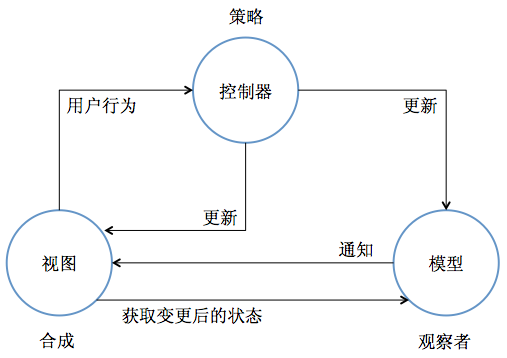
\includegraphics[bb=0 0 513 355, scale=0.45]{figure/fig_n01.png}
		\caption{传统MVC设计模式下各模块交互图}
		\label{fig:n01}
	\end{figure}

  而Cocoa框架(将于下一节“客户端开发框架:Cocoa”中进行介绍)提出尽量保持视图和模型的重用,避免视图和模型之间的交互,转而让控制器来完成,从而保持视图和模型之间的独立,也增强了可重用度。改进的MVC设计模式下各模块交互图如下:

  \begin{figure}[htbp]
		\centering
		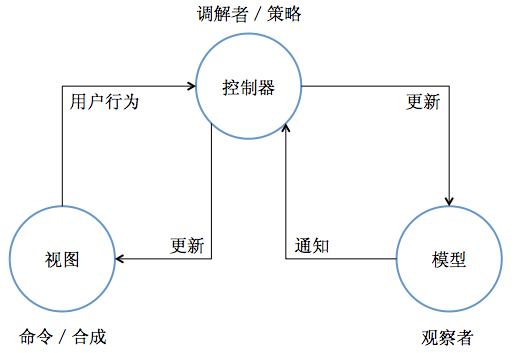
\includegraphics[bb=0 0 510 359, scale=0.45]{figure/fig_n02.png}
		\caption{Cocoa框架中的MVC设计摸下各模块交互图}
		\label{fig:n02}
	\end{figure}

  在该设计模式中,控制器将调解者(mediator)模式和策略模式进行了合并,从而调解视图和模型双向的数据流动。而通过视图对模型状态的变更,也就通过控制器来传达。另外,视图还通过实现Cocoa框架下的对象-行为(target-action)机制,结合了命令模式和合成模式。\cite{iOSLIB} 

	\subsubsection{单例设计模式}
  单例模式,也叫单子模式,是一种常用的软件设计模式。在应用这个模式时,单例对象的类必须保证只有一个实例存在。许多时候整个系统只需要拥有一个的全局对象,这样有利于我们协调系统整体的行为。比如在某个服务器程序中,该服务器的配置信息存放在一个文件中,这些配置数据由一个单例对象统一读取,然后服务进程中的其他对象再通过这个单例对象获取这些配置信息。这种方式简化了在复杂环境下的配置管理。

  实现单例模式的思路是:一个类能返回对象一个引用(永远是同一个)和一个获得该实例的方法(必须是静态方法,通常使用getInstance这个名称);当我们调用这个方法时,如果类持有的引用不为空就返回这个引用,如果类保持的引用为空就创建该类的实例并将实例的引用赋予该类保持的引用;同时我们还将该类的构造函数定义为私有方法,这样其他处的代码就无法通过调用该类的构造函数来实例化该类的对象,只有通过该类提供的静态方法来得到该类的唯一实例。\cite{WIKI}

	\subsection{客户端开发框架:Cocoa}
  Cocoa框架是苹果公司为Mac OS X(包括优化了的适用于移动设备的iOS系统)所创建的原生面向对象的编程环境,是Mac OS X上五大API之一。Cocoa框架包含开发Mac OS X所需的类库、API和运行环境。通过Cocoa框架,开发人员可以以开发Mac OS X的方式进行项目的开发,而且开发出来的应用将自动继承Mac OS X的基本功能并遵循苹果公司的人机界面准则,而且还可以直接可以访问功能强劲的Unix系统底层\cite{Cocoa}。此外,Cocoa框架还遵循MVC的设计模式。

	\subsection{服务器端开发框架:Bottle}
  Bottle是一个小巧的Python Web开放框架,它快速、简单、轻量。Bottle只作为一个简单的文件模块进行发布,除了Python基本库,它不依赖任何第三方库。\cite{N01}

  Bottle支持带参数的URL请求调度,非常方便编写RESTful Web服务。另外,Bottle内置一个HTTP服务器以及为许多第三方WSGI/HTTP服务提供的适配器。一个简单的使用Bottle编写的“Hello World”如下:

  from bottle import route, run

  @route('/hello/:name')
  def hello(name):
      return '<h1>Hello %s!</h1>' % name.title()

  run(host='localhost', port=8080)
  图:Bottle中的“Hello World”程序代码

  通过本地访问http://localhost:8080/hello/foo,可以快速的获得反馈:Hello foo。其中foo可为任意字符串名。

	\subsection{RESTful Web服务}
  REST(Representational state transfer,即表述性状态转移)是Roy Fielding博士在2000年他的博士论文\cite{N02}中提出来的一种软件架构风格。采用REST模式的Web服务相比复杂的SOAP和XML-RPC来说非常的简洁。REST从资源的角度来观察整个网络,由URI来确定分布在各处的资源,客户端也是通过URI来获取资源的表述,从而致使客户端应用程序转变其状态。REST提供了一组架构约束,当作为一个整体来应用时,强调组件交互的可伸缩性、接口的通用性、组件的独立部署、以及用来减少交互延迟、增强安全性、封装遗留系统的中间组件。

  RESTful Web服务(也称为RESTful Web API)是一个使用HTTP并遵循REST原则的Web服务。

	\subsection{弹性云存储服务:Amazon EC2}
  Amazon提供的弹性云计算服务(Elastic Compute Cloud,简称EC2)是一个提供可调整云计算能力的Web服务。它的简单Web服务接口允许用户轻松获取和配置云计算性能,在提供高效稳定的服务环境的同时,还向用户提供了计算资源的完全控制权限。Amazon EC2可减少用户获取和启动新的服务器实例所需的时间,从而可以快速地改变(不管是增加还是减少)计算性能需求的变化。\cite{AWS}

  快速全球部署、按需要使用计费,以及可靠的基础架构正是Amazon EC2的突出的优点。

	\subsection{键值存储服务:Redis}
  Redis\cite{N07}是一个键值(key-value)存储服务系统,全称REmote DIctionary Service。同Memcached类似,它支持存储包括string(字符串)、list(链表)、set(集合)、zset(有序集合)和hash(哈希)在内的值类型。这些数据类型都支持push/pop、add/remove及交并集和差集的操作,而且这些操作都是原子性的。在此基础上,redis还支持各种不同方式的排序。为了保证数据读取效率,redis将数据都缓存于内存中,然后周期性的把更新的数据写入到磁盘(或者可以选择将修改操作追加到日志文件),并且还可在此基础上实现主从(master-slave)同步,从而有效降低灾难性的数据损坏或丢失情况所带来的损失。

  虽然键值数据库还没有完全成熟,但它的确为开发分布式和弹性Web应用提供了很好的选择\cite{N06}。Redis主体结构就是实现一个hash table,它定位于一个内存数据库,正是由于内存的快速访问特性,才使得Redis能够有如此高的性能,能够轻松处理大量复杂的数据结构。

  而对于持久化存储问题,redis提供了RDB(Redis DB)快照和AOF(Append Only File)日志两种策略:

	\subsubsection{RDB快照}
	Redis支持将当前数据的快照存成一个数据文件的持久化机制。而一个持续写入的数据库如何生成快照呢。Redis借助了fork命令的copy on write机制。在生成快照时,将当前进程fork出一个子进程,然后在子进程中循环所有的数据,将数据写成为RDB文件。
  Redis的RDB文件不会坏掉,因为其写操作是在一个新进程中进行的,当生成一个新的RDB文件时,Redis生成的子进程会先将数据写到一个临时文件中,然后通过原子性rename系统调用将临时文件重命名为RDB文件,这样在任何时候出现故障,Redis的RDB文件都总是可用的。
  同时,Redis的RDB文件也是Redis主从同步内部实现中的一环。
	\subsubsection{AOF日志}
	AOF日志是一个追加写入的日志文件。与一般数据库日志不同的是,AOF文件是可识别的纯文本,它的内容就是一个个的Redis标准命令。
  然而,如果每一条写命令都生成一条日志,那么AOF文件将会变得非常大。所以,Redis又提供了一个AOF Rewrite的功能,它将重新生成一份AOF文件,新的AOF文件中一条记录的操作只会有一次,而不像一份老文件那样,可能记录了对同一个值的多次操作。其生成过程和RDB类似,也是fork一个进程,直接遍历数据,写入新的AOF临时文件。在写入新文件的过程中,所有的写操作日志还是会写到原来老的AOF文件中,同时还会记录在内存缓冲区中。当重完操作完成后,会将所有缓冲区中的日志一次性写入到临时文件中。然后调用原子性的rename命令用新的AOF文件取代老的AOF文件。

  RDB和AOF操作都是顺序IO操作,性能都很高。而同时在通过RDB文件或者AOF日志进行数据库恢复的时候,也是顺序的读取数据加载到内存中,所以也不会造成磁盘的随机读。

  此外,redis还支持pipeline模式,其具体过程是客户端一次性发送N个命令,然后等待这N个命令的返回结果被一起返回,从而减少网络I/O次数。该模式下,服务端将命令结果放进queue,再返回给客户端。

	\subsection{反向地理编码技术}
  基于位置服务的数据往往是对应于用户当前位置在地球上的经纬度值,这些经纬度坐标值虽然可以很精确方便地应用与代码中,但是对于用户来说显得并不那么直观。相比坐标值,用户更容易了解与该地理位置相关的特殊信息,比如街道、城市、洲或者国家。\cite{iOSLIB}

  Cocoa框架下的Core Location库中包含Geocoder对象,该对象使用网络服务对经纬度和位置标记(placemark)进行相应的转换。而方向地理编码(reverse geocoding)就是将经纬度坐标转换成位置标记的过程。如图所示为反向地理编码流程示意图:

  \begin{figure}[htbp]
		\centering
		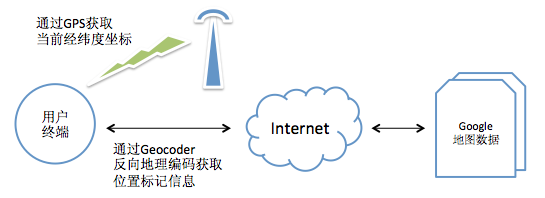
\includegraphics[bb=0 0 788 288, scale=0.45]{figure/fig_n03.png}
		\caption{反向地理编码流程图}
		\label{fig:n03}
	\end{figure}

	\subsection{开发环境}
  操作系统:Mac OS X 10.7.3
  开发工具:Vim 7.3和Xcode 4.2
  Web服务运行环境:Amazon EC2 Ubuntu 11.10

	\subsection{主要开发语言}
  客户端采用Objective-C进行开发。

  Objective-C是由科学家、软件工程师Brad Cox于20世纪80年代早期编写的。它的设计方式是将Smalltalk语言的功能特性引入到C语言的编程环境中。iPhone的框架库中的大部分都是用Objective-C编写的,不过因为这种语言被设计为兼容C语言,所以也可以在应用程序中使用C和C++。Objective-C的主要应用平台是Mac OS X和GNUstep(一个开源的自由OpenStep环境)。\cite{B03}

  服务器端采用Python进行开发。

  Python是一种即译式的、互动的、面向对象的编程语言。它包含了模组式的操作,异常处理,动态资料形态,十分高层次的动态资料结构,以及类别的使用。Python揉合了简单的语法和强大的功能。它的语法表达优美易读。它具有很多优秀的脚本语言的特点:解释的,面向对象的,内建的高级数据结构,支持模块和包,支持多种平台,可扩展。而且它还支持交互式方式运行,图形方式运行。它拥有众多的编程界面支持各种操作系统平台以及众多的各类函数库。利用C和C++可以对它进行扩充。个别的应用软件如果需要有一个可程序化界面也可以利用它来做为扩展语言用。最后,Python的可移植度非常高:它可以在许多的Unix类平台上运行,在Mac、MS-DOS、Windows、Windows NT、OS/2、BeOS,以至RISCOS上都有相关的Python版本。\cite{B05}

	\subsection{本章小结}
  本章介绍了客户端和服务器端开发相关的方法和技术,包括MVC、单例设计模式、Cocoa框架、Bottle框架以及弹性云存储服务、键值数据服务和反向地理编码技术。最后描述了开发环境和主要开发语言。

%-----------------------------------------------------------------------

	\section{游戏总体设计}
	\subsection{设计概要}
  鉴于国内外LBS技术的研究和发展现状,在采用以LBS为核心技术的基础上,实现口袋妖怪类游戏的服务端和客户端的设计与实现。通过将现实世界中的地理位置与游戏虚拟世界相结合,开发基于位置服务的口袋妖怪类游戏。该游戏以经典口袋妖怪游戏为原型,运行于iOS平台上,并且结合了位置服务,口袋妖怪分布在真实的世界中。在不同的城市、国家,用户可以遇到不同的口袋妖怪。

	\subsubsection{游戏类别}
  游戏类别为真人角色扮演类游戏。用户扮演原经典口袋妖怪中的主角,进行全世界的口袋妖怪的收集。

	\subsubsection{游戏面向对象}
  游戏支持所有iOS 5.0及以上系统的iPhone、iPod Touch用户。

	\subsection{整体框架}
  通过验证后的用户首先获取个人相关数据存储到客户端。然后通过开启位置服务,每隔一定时间通过GPS获取当前经纬度坐标,然后通过反向地理编码获得当前位置的标记信息。之后向服务器发送请求,获取当前区域下的数据信息,同时从获得的数据中检索匹配的区域代码,发送到服务器获取对应的野生口袋妖怪数据,之后用户每移动一定距离,通过区域代码生成野生口袋妖怪。每次与野生口袋妖怪的战斗结束后,将客户端数据与服务端数据进行同步,同时检测用户区域是否有大的变化,并相应做出更新操作。整体框架图如图所示:

  \begin{figure}[htbp]
		\centering
		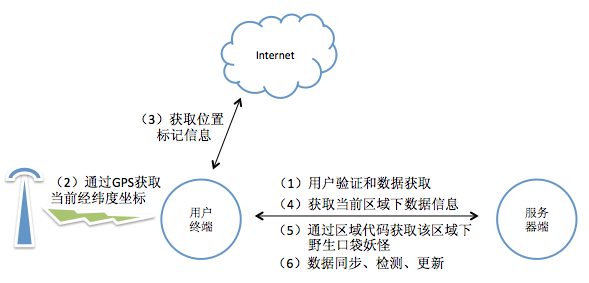
\includegraphics[bb=0 0 582 280, scale=0.45]{figure/fig_n04.png}
		\caption{游戏整体框架图}
		\label{fig:n04}
	\end{figure}

	\subsection{主要功能结构}
  游戏分为客户端和服务器端两个部分。客户端应该有用户的注册和session检测、获取用户数据、获取当前位置的野生口袋妖怪数据、更新用户当前地理位置、数据本地浏览、游戏设置和反馈等主要功能。其功能结构框架图如图所示:

  \begin{figure}[htbp]
		\centering
		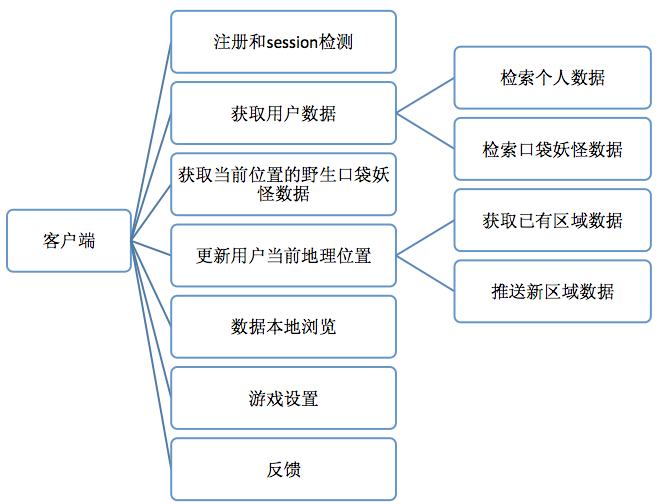
\includegraphics[bb=0 0 651 500, scale=0.45]{figure/fig_n05.png}
		\caption{客户端功能结构框架图}
		\label{fig:n05}
	\end{figure}

  对应的,服务器端应该实现用户个人数据、口袋妖怪数据、野生口袋妖怪数据以及区域数据的基本处理功能。其功能结构框架图如图所示:

  \begin{figure}[htbp]
		\centering
		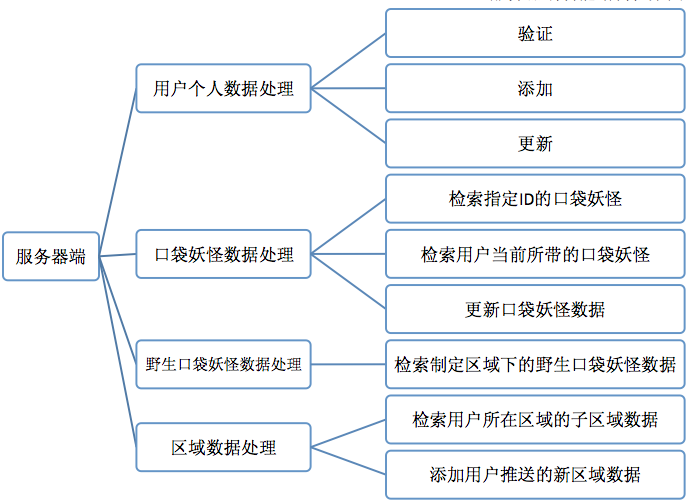
\includegraphics[bb=0 0 693 500, scale=0.45]{figure/fig_n06.png}
		\caption{服务器端功能结构框架图}
		\label{fig:n06}
	\end{figure}

	\subsection{游戏运行流程}
  用户通过OpenID登陆Google Account,成功授权后,客户端发送请求到服务端,如果识别到为新用户,则通过redis的INCR\cite{N08}操作,生成用户ID作为key,用户身份信息作为value,通过redis的SADD操作,将用户信息加入到用户集合中,同时为用户生成默认数据。之后用户可以直接通过识别信息(identity)来获取服务端用户数据、基于地理位置的口袋妖怪数据等。游戏运行的简单流程图如图所示:

  \begin{figure}[htbp]
		\centering
		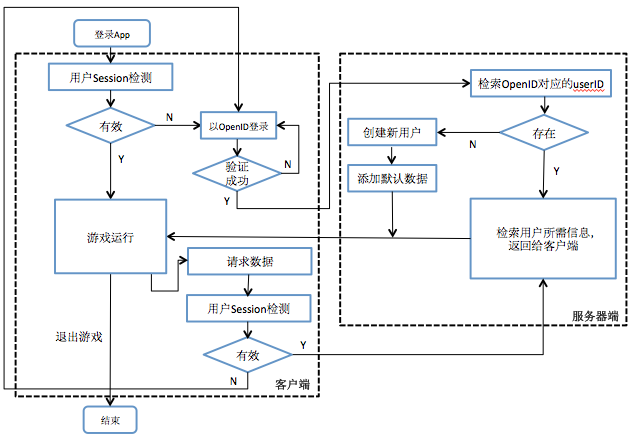
\includegraphics[bb=0 0 955 669, scale=0.45]{figure/fig_n07.png}
		\caption{游戏运行流程图}
		\label{fig:n07}
	\end{figure}

	\subsection{数据库设计}
	\subsubsection{客户端数据库设计}
  客户端采用CoreData作为客户端数据服务,Sqlite3作为数据库保存用户本地数据。各数据实体(在CoreData中称entity,即数据表)如下所示:

  表:客户端数据实体对照表
  \begin{enumerate}
		\item Trainer:用户(训练师)实体
		\item Pokemon:口袋妖怪基本数据实体
		\item TrainerTamedPokemon:捕获口袋妖怪数据实体
		\item WildPokemon:野生口袋妖怪数据实体
		\item Move:口袋妖怪基本技能数据实体
		\item Ability:口袋妖怪基本特性数据实体
		\item BagItem:背包项目实体
		\item Region:区域数据实体
  \end{enumerate}

  Trainer实体可包含多个BagItem实体和TrainerTamedPokemon实体。TrainerTamedPokemon实体和WildPokemon实体均对应一个Pokemon实体,作为其基本数据。而每个Pokemon实体拥有一个Ability实体和四个Move实体。最后,Region实体单独存储,只用于存储和检索区域相关数据。各数据实体关系图如下:

  \begin{figure}[htbp]
		\centering
		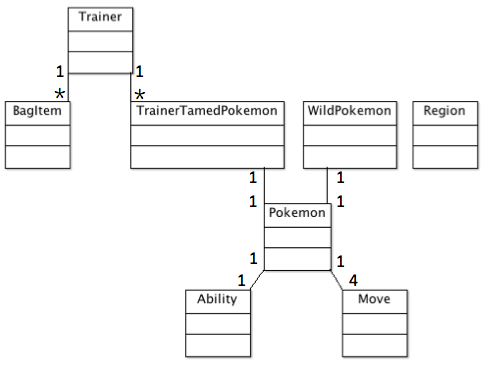
\includegraphics[bb=0 0 486 367, scale=0.45]{figure/fig_n08.png}
		\caption{数据实体关系图}
		\label{fig:n08}
	\end{figure}
  
	\subsubsection{服务器端数据库设计}
  服务器端采用键值数据服务Redis作为数据库,鉴于其运行于内存上,所以拥有很高的性能,能够快速响应用户请求。在Redis的配置上,选择每隔一段时间将内存中的数据写入到磁盘,作为数据永久化保存策略。Redis数据库中各关键字及其值类型和说明如下:

  表:服务器端数据实体对照表
  \begin{enumerate}
		\item global:nextUserid:String:全局用户ID:作为计数器,每次添加新用户时增加1作为用户ID
		\item <provider>:<identity>:String:用户ID:<provider>为第三方OpenID服务对应的ID,<identity>为用户特征字符串
		\item users:Set:用户ID:所有用户ID
		\item usernames:Set:用户名:保证用户用户名唯一性
		\item u:<userid>:多值hash:用户数据:通过用户ID获取用户数据
		\item pm:<userid>:<pokemonid>:多值hash:口袋妖怪数据:获取指定用户的指定口袋妖怪ID的数据
		\item pokedex:<userid>:Set:口袋妖怪ID集:获取指定用户的口袋妖怪图鉴的所有ID
		\item wpm:DEFAULT:String:口袋妖怪ID序列:为未知区域提供的默认野生口袋妖怪ID序列
		\item wpm:<code>:String:口袋妖怪ID序列:通过区域代码获取当前区域下特殊的野生口袋妖怪ID序列
		\item re:<code>:Set:区域数据:通过区域代码获取当前区域下子区域数据
		\item nre:<code>:Set:区域数据:通过区域代码添加新区域数据
  \end{enumerate}

  每添加一个新用户,redis对键global:nextUserid对应的值进行INCR操作生成用户ID。INCR是一个针对字符串的操作,因为redis没有专用的整数类型,所以键内储存的字符串被解释为十进制64位有符号整数来执行INCR操作。

	\subsection{本章小结}
  本章主要对游戏进行了总体的概要设计。明确了游戏的使用对象、大致功能结构及整体框架,在此基础上对游戏的主要功能结构、游戏运行流程进行了初步设计,并对客户端和服务器端的数据库设计进行了简单的介绍。

%-----------------------------------------------------------------------

	\section{游戏详细设计}
	\subsection{项目开发规范}
	\subsubsection{目录规划}
  客户端通过Xcode进行项目的开发和管理,如图所示为项目目录:

  \begin{figure}[htbp]
		\centering
		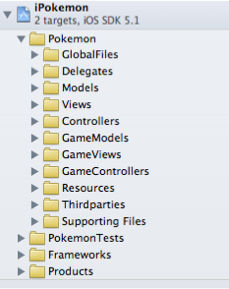
\includegraphics[bb=0 0 229 289, scale=0.45]{figure/fig_n09.png}
		\caption{客户端项目目录}
		\label{fig:n09}
	\end{figure}
  
  客户端项目目录规划表如下:
  
  \begin{enumerate}
		\item Pokemon/:项目主要目录
		\item Pokemon/GlobalFiles/:全局文件,如常量、一些共享类
		\item Pokemon/Delegates/:委托类
		\item Pokemon/Models/:模型类
		\item Pokemon/Views/:视图类
		\item Pokemon/Controllers/:控制器类
		\item Pokemon/GameModels/:游戏部分的模型类
		\item Pokemon/GameViews/:游戏部分的视图类
		\item Pokemon/GameControllers/:游戏部分的控制器类
		\item Pokemon/Resources/:游戏资源
		\item Pokemon/Thirdparties/:第三方库文件
		\item Pokemon/Supporting Files/:项目基本文件
		\item PokemonTests/:测试类
		\item Frameworks/:所有框架
		\item Products/:二进制可运行文件
  \end{enumerate}

  相比客户端,服务器端项目目录非常的简洁:
  \begin{enumerate}
    \item server.py:服务端程序
    \item dump.rdb:Redis数据库
		\item bottle.py;Bottle框架库
  \end{enumerate}

  另外,服务器端系统中,将redis的配置文件redis.conf保存在/etc/目录下。

	\subsubsection{命名规则}
  客户端文件命名,以及类、方法、变量等的命名,均遵循《Google Objective-C Style Guide》的规范,详细命名规则请参阅《Google Objective-C Style Guide》\cite{N03}。

  服务端相关命名则遵循《Google C++ Style Guide》的规范,详细请参阅《Google C++ Style Guide》\cite{N04}。

	\subsection{客户端设计与实现}
  客户端主要以UIKit为主进行设计与实现,辅之采用精灵(sprite\cite{B06})作为游戏战斗场景下口袋妖怪个体进行动画的渲染。

	\subsubsection{视图层次关系}
  如图所示为客户端视图整体层次关系(各视图均对应含有一个控制器,比如MainView对应的控制器为MainViewController):

  \begin{figure}[htbp]
		\centering
		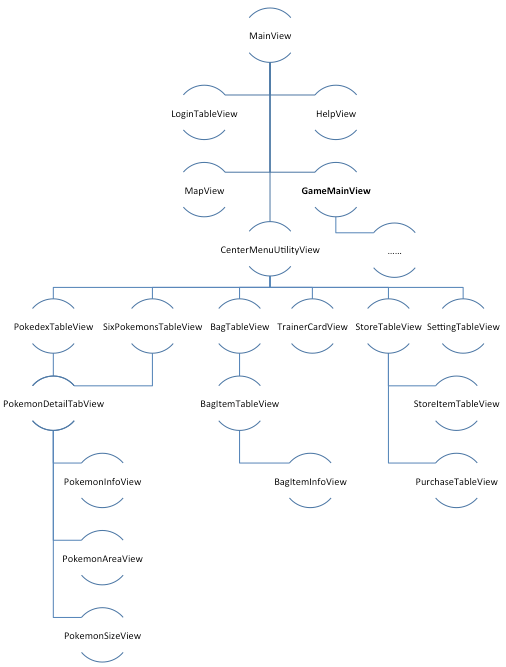
\includegraphics[bb=0 0 506 667, scale=0.45]{figure/fig_n10.png}
		\caption{视图整体层次关系}
		\label{fig:n10}
	\end{figure}

  MainView为主视图,它包括五个主要子视图:LoginTableView(登录视图)、HelpView(帮助视图)、MapView(地图)、GameMainView(游戏主视图)、CenterMenuUtilityView(主菜单视图)。其各功能如下:

  \begin{enumerate}
		\item LoginTableView:当用户session无效时显示给用户,提供第三方验证服务进行登;
		\item HelpView:用户帮助视图;
		\item MapView:地图,用户可查看自己所在位置,以及周边口袋妖怪情况等信息;
		\item GameMainView:游戏战斗主视图,当用户遇到野生口袋妖怪时,进入战斗场景;
		\item CenterMenuUtilityView:主菜单视图,包含六个子菜单:PokedexTableView(图鉴列表视图)、SixPokemonsTableView(用户所带口袋妖怪列表视图)、BagTableView(背包列表视图)、TrainerCardView(用户信息视图)、StoreTableView(商店视图)、SettingTableView(设置视图)。
  \end{enumerate}

  此外,GameMainView还包含一系列子视图,其层次关系如图所示:

  \begin{figure}[htbp]
		\centering
		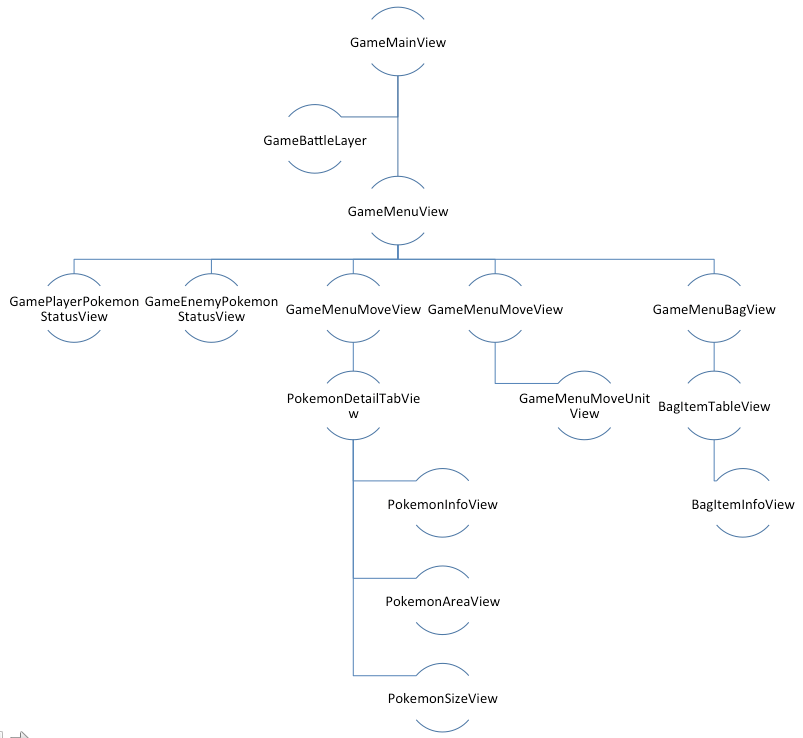
\includegraphics[bb=0 0 803 738, scale=0.45]{figure/fig_n11.png}
		\caption{GameMainView子视图层次关系}
		\label{fig:n11}
	\end{figure}

  所有视图对应的控制器调解视图的显示与更新、数据模型的获取与更新,以及视图与模型之间的通信。

	\subsubsection{数据模型}
  模型(在Cocoa中也称为entity,实体)主要有:Trainer(训练师,即用户)、TrainerTamedPokemon(训练师捕获的口袋妖怪)、WildPokemon(野生口袋妖怪)、Pokemon(口袋妖怪)、BagItem(背包物品)、Region(区域)、Move(口袋妖怪技能)、Ability(口袋妖怪特性)。

  Trainer、TrainerTamedPokemon、WildPokemon为动态模型,控制器可以检索当前相关数据,并对其进行更新后保存。而Pokemon、BagItem、Move、Ability为静态模型,控制器只检索相关数据,不对其进行更新。

  Trainer、TrainerTamedPokemon、WildPokemon模型相关类图如下:

  \begin{figure}[htbp]
		\centering
		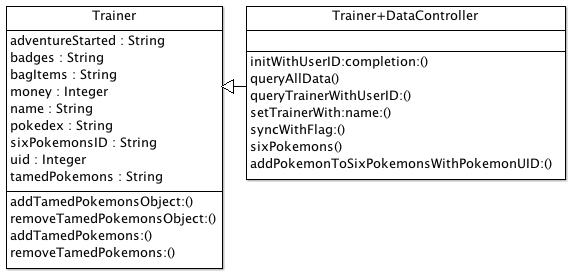
\includegraphics[bb=0 0 570 273, scale=0.45]{figure/fig_n12.png}
		\caption{Trainer模型相关类图}
		\label{fig:n12}
	\end{figure}

  \begin{figure}[htbp]
		\centering
		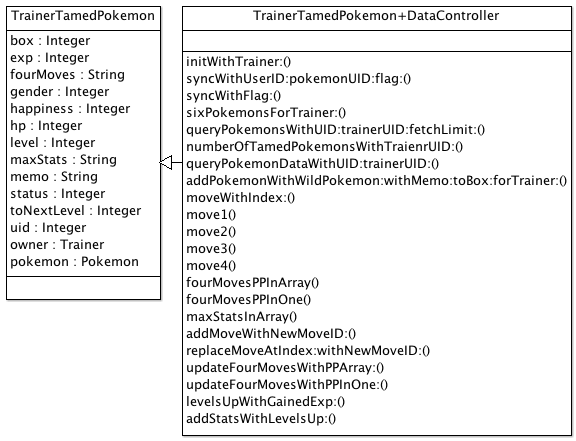
\includegraphics[bb=0 0 576 440, scale=0.45]{figure/fig_n13.png}
		\caption{TrainerTamedPokemon模型相关类图}
		\label{fig:n13}
	\end{figure}

  \begin{figure}[htbp]
		\centering
		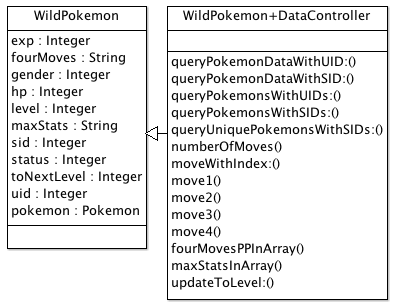
\includegraphics[bb=0 0 391 304, scale=0.45]{figure/fig_n14.png}
		\caption{WildPokemon模型相关类图}
		\label{fig:n14}
	\end{figure}

  Category(扩展类)为Objective-C中包含的特殊的类扩展方式,即该类在拥有相同的属性和方法的同时,可以添加更多方法,从而达到扩展类的作用,而类名不变。Category不能给类添加实例变量,只能添加方法\cite{B07}。比如Trainer类,其扩展类为Trainer+DataController类(可被称为模型控制器),前者的方法只负责数据的增加、删除和更新,而后者在前者的基础上添加了数据检索相关方法,为其它控制器提供了方便的接口,也提升了重用度。在具体编程中,只需要加入Trainer+DataController.h文件,然后便可以对Trainer类使用扩展的方法了。类似的,TrainerTamedPokemon和WildPokemon也进行了相应的扩展。

  TrainerTamedPokemon和WildPokemon模型中属性pokemon为Pokemon类,关系为一对一。Pokemon模型为静态模型,只提供数据索引,其相关类图如下:

  \begin{figure}[htbp]
		\centering
		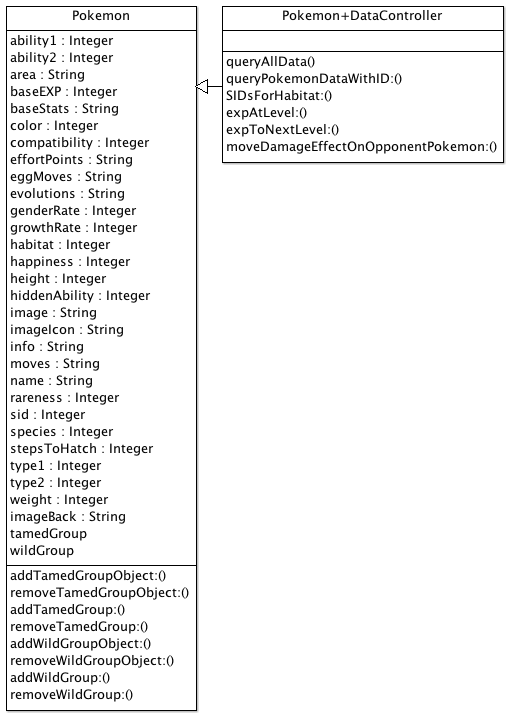
\includegraphics[bb=0 0 508 715, scale=0.45]{figure/fig_n15.png}
		\caption{Pokemon模型相关类图}
		\label{fig:n15}
	\end{figure}

  而对于BagItem、Move、Ability,可分别通过SID号索引静态数据。

  Region为游戏提供基于位置的相关数据,具体数据处理机制将在“基于位置服务的口袋妖怪分布机制”一章中进行详细的介绍。其模型相关类图如下:

  \begin{figure}[htbp]
		\centering
		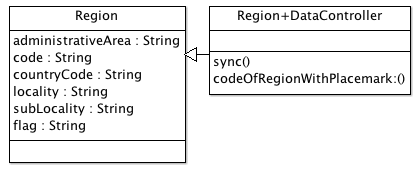
\includegraphics[bb=0 0 420 175, scale=0.45]{figure/fig_n16.png}
		\caption{Region模型相关类图}
		\label{fig:n16}
	\end{figure}

  Region+DataController类同样为Region进行了扩展,为检索和同步数据提供了简单的接口。

	\subsubsection{单例}
  在客户端中,为方便游戏的全局控制,设计了一系列单例:PMAudioPlayer、LoadingManager、ServerAPIClient、OAuthManager、PMLocationManager、TrainerController、WildPokemonController,以及GameStatusMachine、GameSystemProcess、GamePlayerProcess、GameEnemyProcess。

  所有单例获取方法(sharedInstance)除返回类型不同,其它都相同。如OAuthManager单例获取方法如下:
  \begin{figure}[htbp]
		\centering
		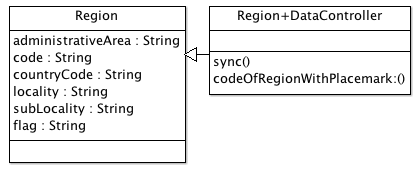
\includegraphics[bb=0 0 420 175, scale=0.45]{figure/fig_n16.png}
		\caption{OAuthManager单例获取方法代码}
		\label{fig:n16}
	\end{figure}

  PMAudioPlayer、LoadingManager、ServerAPIClient、OAuthManager、PMLocationManager各功能如下:

  \begin{enumerate}
		\item PMAudioPlayer:对背景音乐、音效进行全局控制;
		\item LoadingManager:控制同步、异步加载;
		\item ServerAPIClient:提供与服务端交互的接口,包括获取和更新用户ID、数据,区域信息等;
		\item OAuthManager:提供用户验证、session检测、注销等接口;
		\item PMLocationManager:监听用户在地理位置上的移动,适时地更新地理位置标记信息。
  \end{enumerate}

  TrainerController提供当前用户所有包括个人信息、背包数据、捕获的口袋妖怪相关数据等在内的数据处理接口,此外还包括用户的验证、与服务端数据的同步等接口。其相关类图如下:

  \begin{figure}[htbp]
		\centering
		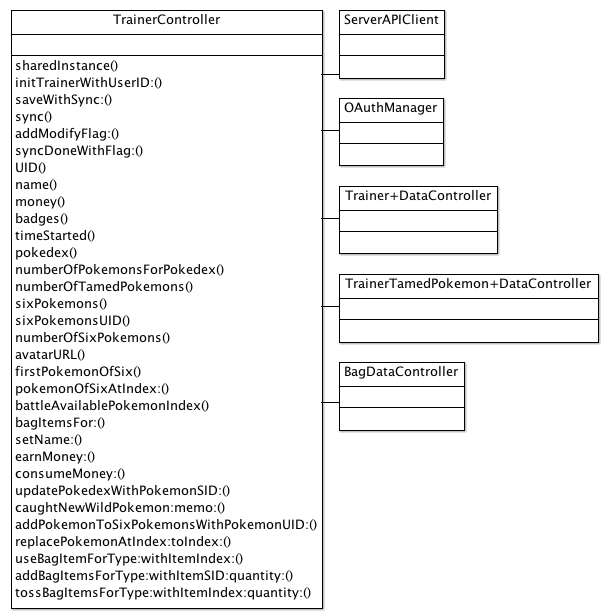
\includegraphics[bb=0 0 604 615, scale=0.45]{figure/fig_n17.png}
		\caption{TrainerController单例相关类图}
		\label{fig:n17}
	\end{figure}

  WildPokemonController根据PMLocationManager获取的用户当前地理位置数据,生成相应的野生口袋妖怪。同时,它包含与服务端数据交互的私有接口。其相关类图如下:

  \begin{figure}[htbp]
		\centering
		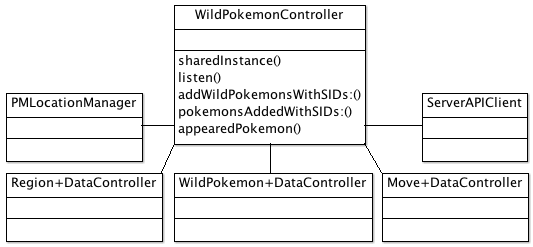
\includegraphics[bb=0 0 533 247, scale=0.45]{figure/fig_n18.png}
		\caption{WildPokemonController单例相关类图}
		\label{fig:n18}
	\end{figure}

  GameStatusMachine为在战斗模式下的状态机,对游戏战斗的回合进行控制。而GameSystemProcess、GamePlayerProcess、GameEnemyProcess均为CCNode子类,包含update:方法来更新游戏,三者分别为系统处理器、用户(玩家)处理器、敌人(野生口袋妖怪)处理器,在游戏回合中各自监听和处理自己的事件。

  \subsection{服务端接口设计与实现}
  服务端以Python语言进行编写,采用轻量级Web服务框架Bottle构建Web服务,提供RESTful Web API。服务器托管于美国西部的加利福尼亚洲,Amazon EC2上运行64位Ubuntu 11.10系统实例,开放22端口(用于管理员通过SSH进行连接管理服务器)和8080端口(用于客户端访问API)。考虑到费用和服务需求之间的关系,选择采用最低性能的实例(Micro Instance),提供613MB内存(可方便进行扩展)。

  用户数据使用Redis v2.4进行存储,采用Redis Python Client(提供Python访问Redis数据的接口)进行数据交互操作。

  主要API设计和说明如下:

  表:服务端Web服务主要API表
  \begin{enumerate}
		\item /id:ID,获取已验证用户的ID
		\item /u:User,获取用户数据
		\item /uu:Update User,更新用户数据
		\item /6pm:Six PokeMons,获取用户所带口袋妖怪数据
		\item /pd:PokeDex,获取用户口袋妖怪图鉴数据
		\item /upm:Update PokeMon,更新口袋妖怪数据
		\item /wpm:Wild PokeMon,获取用户当前区域下可能出现的野生口袋妖怪
		\item /r/<code>:Region,获取指定区域code的区域数据(code示例:CN:ZJ:HZ:XX:XX)
  \end{enumerate}

	\subsection{基于位置服务的口袋妖怪分布机制实现}
  游戏中,口袋妖怪在现实世界中的分布并不是一成不变的,服务器端每隔一定时间更新野生口袋妖怪分布数据,映射到现实世界中。客户端(用户移动设备)通过一定时间间隔或移动一定距离后,发送消息到服务器端,获取当前区域特殊的野生口袋妖怪。野生口袋妖怪的分布除了考虑区域的不同外,还将考虑地形的影响,比如沿海城市出现水系口袋妖怪,沙漠地带出现岩石类口袋妖怪,等等。

  客户端反向地理编码生成对应野生口袋妖怪的主要代码如下:
   \begin{figure}[htbp]
		\centering
		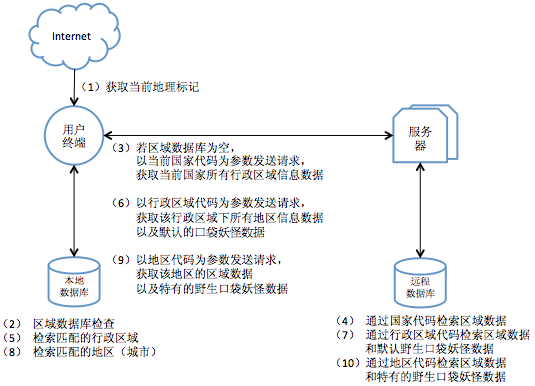
\includegraphics[bb=0 0 749 669, scale=0.45]{figure/fig_n19.png}
		\caption{反向地理编码主要代码}
		\label{fig:n19}
	\end{figure}

  GLGeocoder对象geocoder通过reverseGeocodeLocation:completionHandler:方法,以self.location(经纬度坐标等信息,CLLocation类)发送请求获取当前地理位置信息,当得到回复后,调用completionHandler代码块,对self.locationInfo(当前地理信息,NSDictionary类)和self.regionCode(当前区域代码,NSString类)进行相应的更新。并发送消息给WildPokemonController单例,生成野生口袋妖怪。

  通过反向地理编码获得的地理标记包含国家代码(ISOcountryCoude)、国家名(country)、邮政编码(postalCode)、行政区域名(administrativeArea)、地区名(locality)、次级地区名(subLocality)、是否为内陆水域(inlandWater)、是否为海洋(ocean)等信息。

  地理标记(placemark)各属性和说明如下:

  表:地理标记对照表
  \begin{enumerate}
		\item 属性名 | 说明
		\item addressDictionary | 一个可读的连续地址字典
		\item administrativeArea | 行政区域名
		\item areasOfInterest | 与当前区域相关的有趣的地方
		\item country | 国家名称
		\item inlandWater | 内陆湖泊名称
		\item ISOcountryCode | 国家缩写代码
		\item locality | 地区(城市)名称
		\item location | 一个包含经纬度坐标的CLLocation对象
		\item name | 地理标记名
		\item ocean | 海洋名称(如果所在处为海洋的话)
		\item postalCode | 邮政编码
		\item region | 地理区域范围
		\item subAdministrativeArea | 附加的行政区域信息(可无)
		\item subLocality | 次级地区名(可无)
		\item subThoroughfare | 附加街道信息
		\item thoroughfare | 街道名称
  \end{enumerate}
  
  然而,这些信息也仅仅为显示给用户而设计,也就说,当用户发送请求后,获得的是自己所在位置对应经纬度坐标下的地理信息,然后显示在屏幕上。而如何确定用户所在处,这就需要对获得的信息进行相应的匹配来确定,但苹果公司并没有给出所有地理信息名称,所以需要通过用户来搜集地理信息名称,然后将更新好的地理信息存储到服务器,之后其它用户便可以获取该地理信息数据。具体设计如下:

   \begin{figure}[htbp]
		\centering
		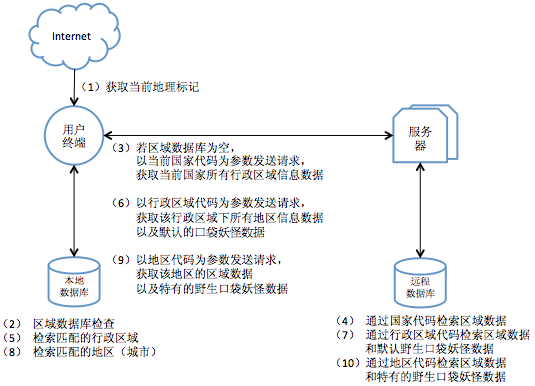
\includegraphics[bb=0 0 749 669, scale=0.45]{figure/fig_n19.png}
		\caption{客户端和服务端交互详细示意图}
		\label{fig:n19}
	\end{figure}

  客户端和服务端各包含一个区域数据库。客户端数据库(本地数据库)存储用户在当前省份下的区域信息,服务端数据库(远程数据库)存储全球区域信息。
  
  当用户登录客户端后,进行区域信息数据初始化工作: 
  
  1. 根据用户当前经纬度坐标,反向地理编码后获得区域信息;
  2. 检查本地区域数据库中是否已初始化;
  3. 若未初始化(即区域数据库为空),则以国家代码\cite{N05}(如中国的国家代码为CN)作为参数向服务端发送请求,以获取该国家下所有行政区域(或省)信息数据;
  4. 服务器端根据请求参数中的国家代码,生成键(如中国对应的为re:CN),从数据库中检索区域数据,返回给客户端;
  5. 客户端通过地理标记检索匹配的行政区域,获得对应的行政区域代码(如中国浙江省为CN:ZJ,若无匹配数据,则以CN:XX代替);
  6. 客户端以行政区域代码为参数向服务器端发送请求,以获取该行政区域下所有地区信息数据,同时获取分布于该行政区域下的默认的野生口袋妖怪数据;
  7. 服务器端根据请求参数中的行政区域代码,生成键(如中国浙江省对应的为re:CN:ZJ),从数据库中检索区域数据,返回给客户端;
  8. 客户端通过地理标记检索匹配的地区(城市),获得对应的地区代码(如中国浙江省杭州市为CN:ZJ:HZ,若无匹配数据,则以CN:ZJ:HZ代替);
  9. 客户端以地区代码为参数向服务器端发送请求,以获取该地区下的区域数据以及该地区下特有的野生口袋妖怪数据;
  10. 服务器端根据请求参数中的地区代码,生成两个键(如中国浙江省杭州市对应的为re:CN:ZJ:HZ和wpm:CN:ZJ:HZ),从数据库中检索该地区下的区域数据和所有野生口袋妖怪数据,返回给客户端;
  
  之后,用户每到一个地方或每隔一定时间,通过更新的地理标记数,客户端向数据库索引匹配的区域数据,对应的根据区域代码(如中国浙江杭州市余姚区对应的为CN:ZJ:HZ:YY),生成野生口袋妖怪数据,并提醒用户出现野生口袋妖怪。主方法如下:

   \begin{figure}[htbp]
		\centering
		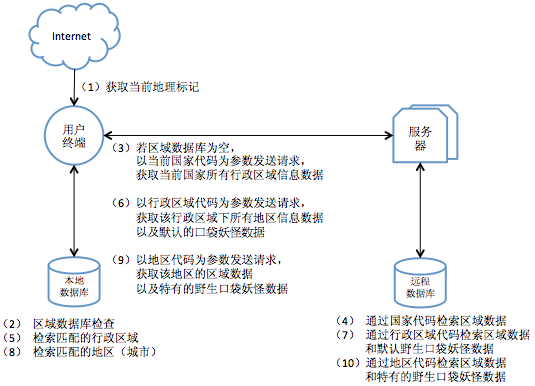
\includegraphics[bb=0 0 749 669, scale=0.45]{figure/fig_n19.png}
		\caption{根据区域生成野生口袋妖怪主方法代码}
		\label{fig:n19}
	\end{figure}

  通过\_updateRegionCodeWithPlacemark:方法(将在下一节介绍)更新区域代码后,从该区域对应的特有的野生口袋妖怪中随机生成一个ID号,然后从本地数据库中获取该野生口袋妖怪的数据。如果没有该野生口袋妖怪的匹配数据,则通过\_updateForCurrentRegion方法从服务器端获取该区域下的数据到本地进行更新。成功生成野生口袋妖怪后,发送消息给用户,提醒有野生口袋妖怪出现。

  但是由于区域数据的不完整性,在客户端从本地数据库中检索区域数据时,可能无法获得匹配的区域数据。这时,系统将当前地理位置下对应的地理标记数据存入本地数据库,将标记(flag)参数设置为n(即新区域信息数据),然后在下次向服务器获取数据的同时,将所有标记为n的区域信息数据推送给服务器,然后将标记重置为p(即地理标记数据已经发送给服务器,下次便不必再进行存储和发送工作)。

  本地区域数据检索与更新的主要代码如下:
   \begin{figure}[htbp]
		\centering
		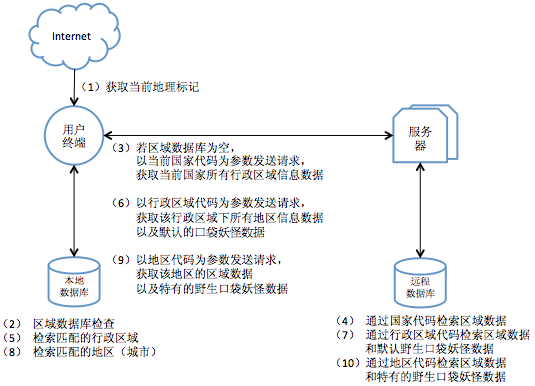
\includegraphics[bb=0 0 749 669, scale=0.45]{figure/fig_n19.png}
		\caption{本地区域数据检索与更新的主要代码}
		\label{fig:n19}
	\end{figure}

  placemark为传入参数,存储当前区域下的地理标记数据。fetchRequest检索本地数据库中locality与placemark.locality相同的数据。若不存在,添加placemark中存储的地理标记数据到数据库中;反之返回匹配的区域代码。

  远程数据库中,对未知行政区域信息,统一存储在国家代码下,比如,中国,获得未知的行政区域名:Heilongjiang(黑龙江),那么,对应在redis中的键值也就是:nre:CN => 'Heilongjiang Province',其中,nre代表新区域(New REgion)作为键前缀,nre:CN对应的值为一个集合;而对未知地区信息,则统一存储在行政区域对应代码下,比如,中国浙江,获得未知的地区名:Shaoxing City(绍兴),那么,对应在redis中的键值也就是:nre:CN:ZJ => 'Shaoxing City'(同样,nre:CN:ZJ对应的值为一个集合);依次类推。

  管理员每隔一段时间对地理信息数据进行维护,抓取所有前缀为nre的键对应的集合,对每条数据进行更新,比如数据:nre:CN:ZJ => 'Shaoxing City',更新后,记代码为CN:ZJ:SX。最后,将所有更新了的数据以re:CN:ZJ:SX => 'CN:ZJ:SX,Zhejiang Province,Shaoxing City'形式存储到数据库中,同时备份删除原先前缀为nre的键对应的数据。

  最后,对区域代码和对应的野生口袋妖怪ID进行键值匹配,设定对应区域下特殊的口袋妖怪。比如中国浙江省杭州市余杭区特有的野生口袋妖怪ID有1,2,3,则对应数据为wpm:CN:ZJ:HZ:YY => '1,2,3',其中,wpm代表野生口袋妖怪(Wild PokeMon)作为键前缀。

  \begin{figure}[htbp]
		\centering
		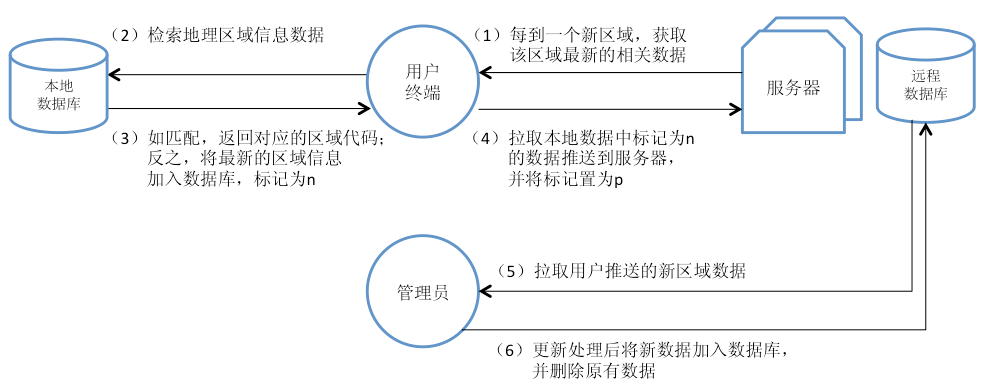
\includegraphics[bb=0 0 786 367, scale=0.45]{figure/fig_n20.png}
		\caption{地理信息数据更新示意图}
		\label{fig:n20}
	\end{figure}

  之后,其它用户在获取区域信息和对应的野生口袋妖怪时,便可以获取到最新的数据信息。

	\subsection{本章小结}
  本章在第五章的基础上对游戏进行了详细设计。首先,在游戏开发之前,对游戏的开发规范,包括目录规划、命名规则等进行了规定。重点介绍游戏客户端和服务端各功能模块的详细设计和实现,最后对口袋妖怪的分布机制的实现进行了详细的介绍。

%-----------------------------------------------------------------------

	\section{游戏实现}
  游戏客户端有简体中文和英文两个版本。

	\subsection{客户端界面}
  游戏客户端界面主要采用Cocoa框架下的UIKit库进行编写。主要视图示例如下:

  \begin{figure}[htbp]
		\centering
		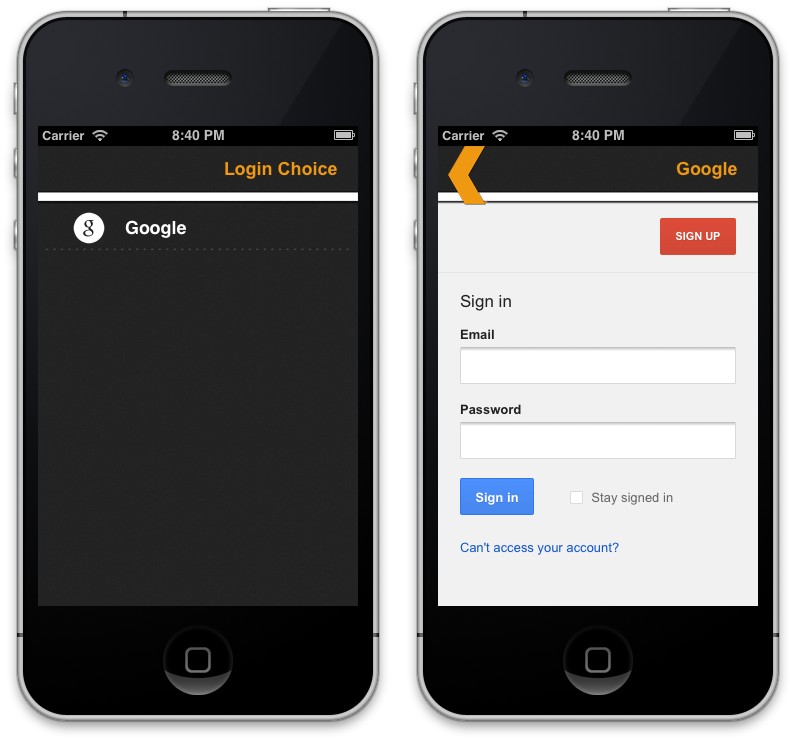
\includegraphics[bb=0 0 790 744, scale=0.45]{figure/fig_n21.png}
		\caption{主视图和主菜单视图}
		\label{fig:n21}
	\end{figure}

  \begin{figure}[htbp]
		\centering
		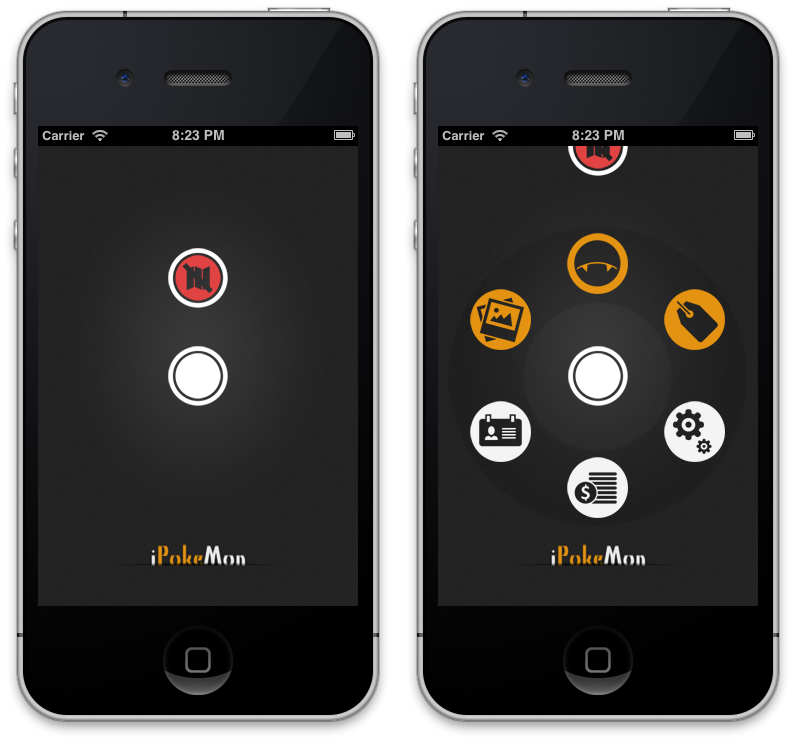
\includegraphics[bb=0 0 790 744, scale=0.45]{figure/fig_n22.png}
		\caption{口袋妖怪图鉴视图和信息视图}
		\label{fig:n22}
	\end{figure}

  \begin{figure}[htbp]
		\centering
		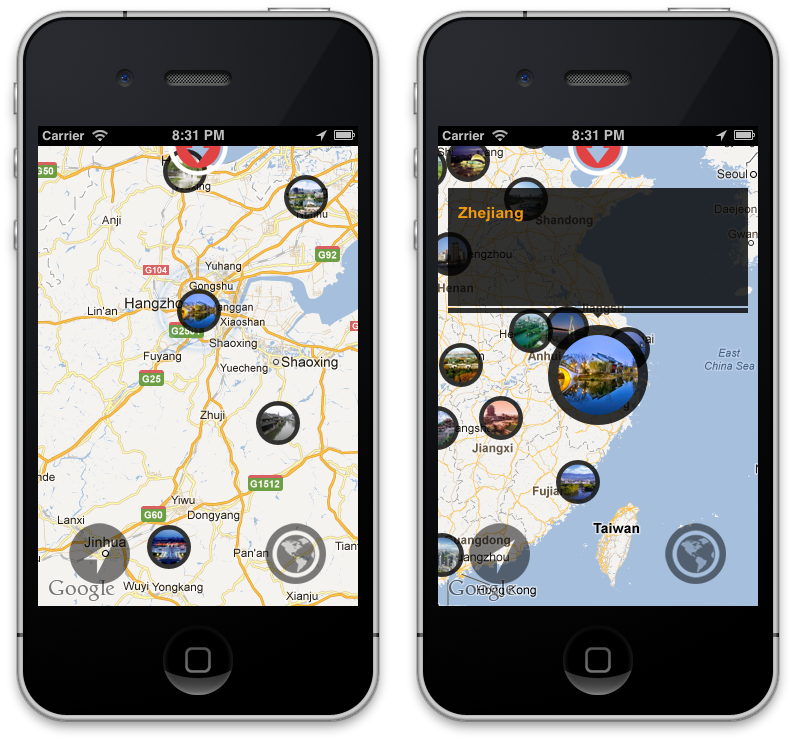
\includegraphics[bb=0 0 790 744, scale=0.45]{figure/fig_n23.png}
		\caption{背包视图和背包项视图}
		\label{fig:n23}
	\end{figure}

  \begin{figure}[htbp]
		\centering
		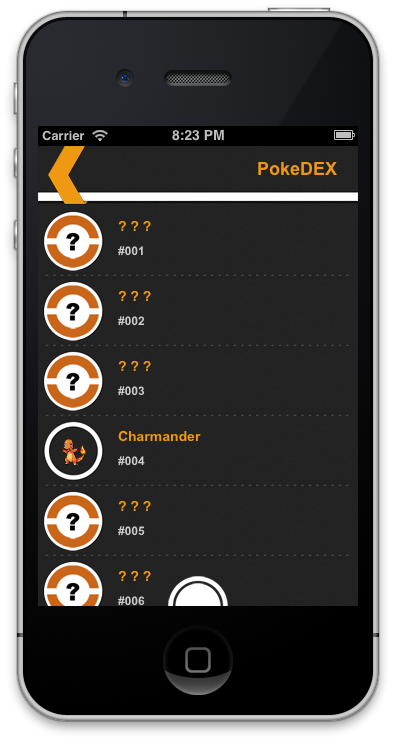
\includegraphics[bb=0 0 790 744, scale=0.45]{figure/fig_n24.png}
		\caption{商店视图和设置页视图}
		\label{fig:n24}
	\end{figure}

  \begin{figure}[htbp]
		\centering
		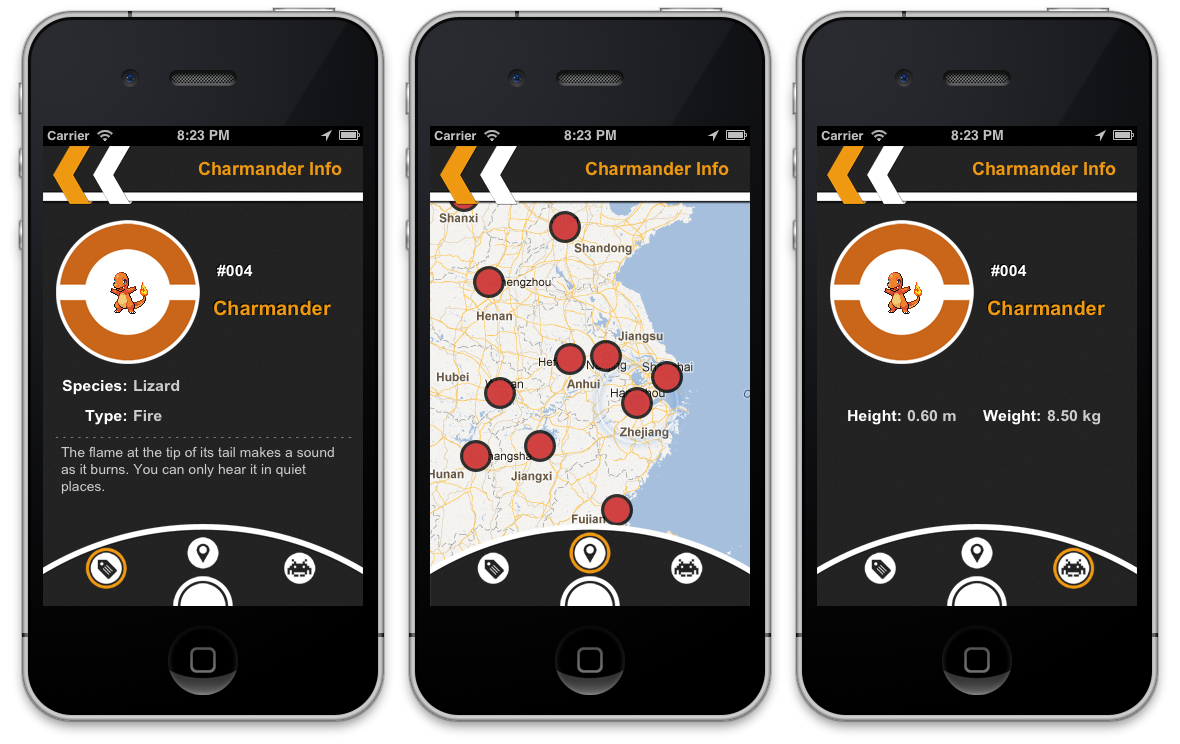
\includegraphics[bb=0 0 790 744, scale=0.45]{figure/fig_n25.png}
		\caption{战斗场景视图和口袋妖怪替换视图}
		\label{fig:n25}
	\end{figure}

	\subsection{基本功能}
  \begin{enumerate}
    \item 可以根据你所在的位置出现不同的口袋妖怪
    \item 如果拥有精灵球,就可以捕获口袋妖怪
    \item 应用可以在后台运行,当出现野生口袋妖怪时,会收到应用的推送信息
    \item 可以使用回复类治疗口袋妖怪
    \item 内置商店,可购买物品
    \item 以及更多原口袋妖怪游戏中存在的一些功能
  \end{enumerate}

	\subsection{操作说明}
  游戏主视图中间的按钮是游戏的主按钮,用户可以通过它打开主菜单。而在它之上的按钮是地图按钮,默认为红色,也就是说位置服务被禁用,用户可以通过按住该按钮保持3秒来开启位置服务,然后按钮会变为白色。

  开启位置服务后,用户可以根据自己当前位置的不同遇到不同的野生口袋妖怪。当有野生口袋妖怪出现时,主按钮会改变状态以示提醒用户。通过按下提醒状态下的主按钮,游戏便加载战斗场景。

  在战斗场景中,用户可以做如下手势操作:

  \begin{enumerate}
    \item 向右滑动手指:展开技能窗口
    \item 向左滑动手指:展开背包窗口
    \item 向上滑动手指:展开你的口袋妖怪的状态栏
    \item 向下滑动手指:展开野生口袋妖怪的状态栏
    \item 轻按底部按钮:展开口袋妖怪选择窗口,用于替换口袋妖怪
    \item 双指连续轻敲两下:尝试逃离战斗
  \end{enumerate}

	\subsection{本章小结}
  本章介绍了游戏最终实现成果,包括游戏客户端界面的实现、基本功能以及操作说明。

%-----------------------------------------------------------------------

  \section{总结与展望位置}
  \subsection{总结}
  论文论述了LBS相关架构和基于位置服务的口袋妖怪类游戏客户端和服务端的设计与实现。客户端采用Cocoa框架,以Objective-C语言编写iPhone客户端游戏程序,通过将现有LBS技术应用于游戏中,将真实世界映射到游戏中,形成一个真实的口袋妖怪世界。采用CoreData作为客户端数据服务,Sqlite3作为数据库保存用户本地数据。服务端托管于Amazon EC2上,采用Python语言编写服务端程序,向客户端提供RESTful Web API,实现了用户验证、获取用户ID和数据、获取用户当前位置下特殊的野生口袋妖怪数据、更新区域位置数据等主要功能。采用键值数据服务Redis作为服务端数据库,鉴于其运行于内存上,所以拥有很高的性能,能够快速响应用户请求。在Redis的配置上,选择每隔一段时间将内存中的数据写入到磁盘,作为数据永久化保存策略。此外,所有客户端和服务端之间的通信,都采用异步编程,数据的传输对用户来说都是透明的。最后,实现了针对iOS平台的基于位置服务的口袋妖怪类游戏。

	\subsection{展望}
  口袋妖怪这款经典游戏深受游戏玩家喜爱,然而由于版权属于任天堂,所以后续开发需要加入自己设计的一套类口袋妖怪的角色和相应的数据,以此避免版权纠纷。Solomo(social-local-mobile,即社交、位置、移动)的应用模式正逐渐被人们肯定。毫无疑问,在位置服务和移动游戏的基础上加入社交元素,将吸引更多的玩家,而社交元素也正是后续考虑加入的。另外,也将加入多人对战、交易等模式,令游戏更具可玩性。相信这款基于位置服务的口袋妖怪类游戏也将深受玩家喜爱。


	\section{致谢}
  在项目和论文完成之际,我要感谢在论文写作和研究期间给予我帮助的老师、同学和朋友们。
  首先要感谢我的指导教师王万良教授和徐新梨副教授。感谢两位在毕业设计期间给予我的悉心指导,为我提供了一个良好的工作和学习环境。他们一丝不苟的工作作风、严谨的治学态度和对工作无私的奉献精神,深深地影响了我,使我受益匪浅。
  再次感谢徐新黎副教授耐心地对我的论文提出修改意见。
  还要感谢我身边和异地的同学、朋友们对我的关心和帮助。
  最后感谢我的父母。感谢他们生活上对我无微不至的照顾与关怀,学业和事业上一如既往的支持与鼓励。
  

	% Import references datas
  \bibliography{references.bib}

	\end{CJK}
\end{document}
